\sub{Lokale Speicherung im Browser}
Der zweite Schritt Daten offline verfügbar zu machen ist sie im Browser zu speichern. Einige Konzepte hierfür werden im Folgenden erläutert.
%
\subsub{Web Storage}
Das Web Storage \gls{API} ist ein Web-Standard mit dessen Hilfe Daten als Schlüssel / Wert Paare im Browser gespeichert werden können. Es wird, wie Abbildung \ref{fig:webStorage} zeigt, von allen relevanten Browsern unterstützt.
Web Storage umfasst zwei Mechanismen. Den Session Storage und den Local Storage.\\
Der Session Storage existiert nur so lange der Browser geöffnet ist.
Das heißt alle Daten die im Session Storage gespeichert werden, existieren nicht mehr sobald der Browser geschlossen wird. Daten die im Local Storage gespeichert sind, existieren dort solange bis der Browser Cache geleert wird~\cite{webstorage}.
\begin{figure}[H]
	\centering
	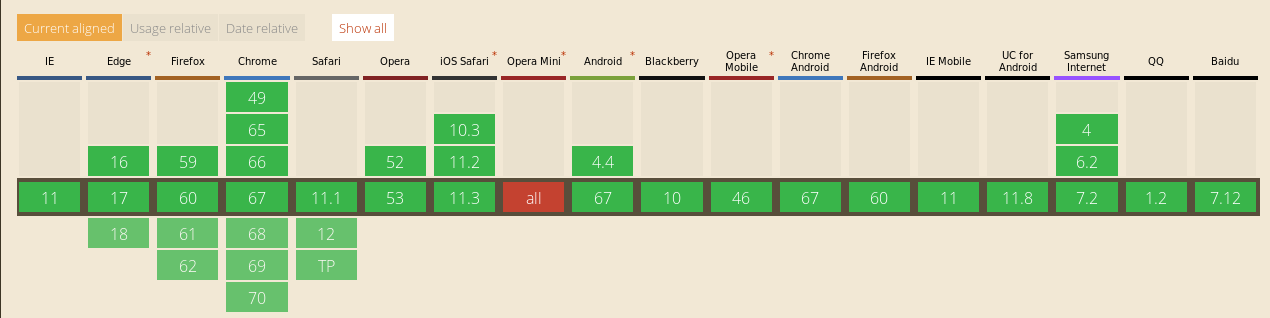
\includegraphics[width=\textwidth]{webStorage}
	\grayRule
	\caption{Browserkompatibilität für Web Storage, Quelle: ~\cite{caniuse-ws}}
	\label{fig:webStorage}
\end{figure}
Der von den Browsern freigegebene Cache-Space für Web Storage variiert, ist aber meist auf 10 MB begrenzt. Der größte Nachteil ist wohl, dass Web Storage synchron arbeitet und so andere Operationen, wie zum Beispiel das Rendern der Seite, blockieren kann~\cite{webstorage-con}.
%
%
\subsub{WebSQL}
Eine andere der lokalen Speicherung im Browser ist die Web SQL Datenbank.
Sie hat ein asynchrones \gls{API} und unterstützt die grundlegenden SQL Abfragen. Web SQL sollte in den W3C Standards aufgenommen werden. Aus Mangel unabhängigen Implementierungen wie eine andere \gls{DB} als SQLite im Backend wurde es abgelehnt~\cite{websql}.\\
Das Web SQL \gls{API} wird nur von den Webkit--Browsern unterstützt. Also nicht von Firefox, dem Internet Explorer oder dessen neueren Variante Edge~\cite{caniuse-websql}.
%
%
\subsub{IndexedDB}
\begin{figure}[H]
	\centering
	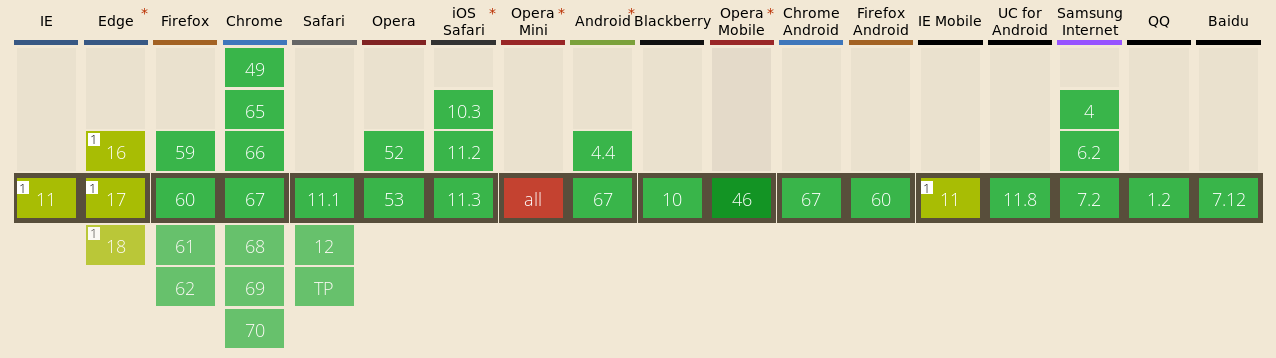
\includegraphics[width=\textwidth]{indexedDB}
	\grayRule
	\caption{Browserkompatibilität für IndexedDB, Quelle: ~\cite{caniuse-idb}}
	\label{fig:indexedDB}
\end{figure}
%
\subsub{IndexedDB 2}
\begin{figure}[H]
	\centering
	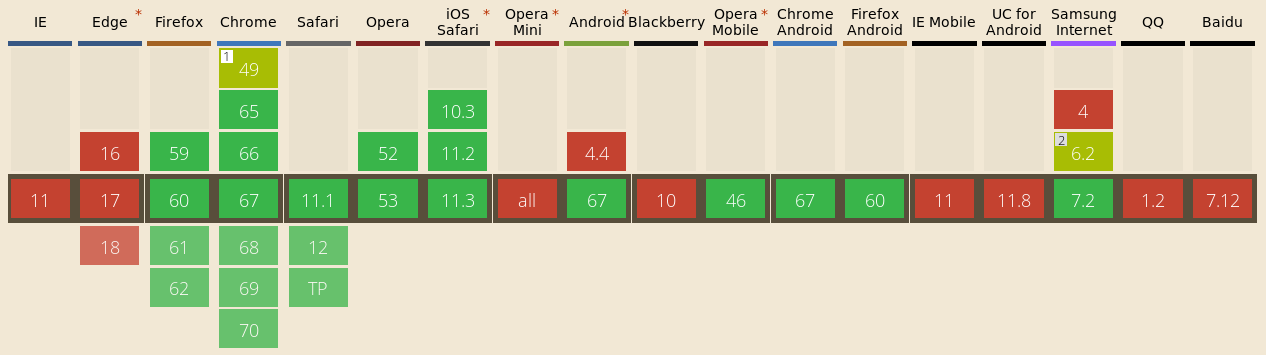
\includegraphics[width=\textwidth]{indexedDB2}
	\grayRule
	\caption{Browserkompatibilität für IndexedDB 2.0, Quelle: ~\cite{caniuse-idb}}
	\label{fig:indexedDB2}
\end{figure}
https://www.w3.org/TR/IndexedDB-2/